% !TeX spellcheck = en_US
% !TEX root = ../thesis-example.tex
%
\section{Closing remark: order of calculation}

The discussed order is written in respect of transformation operations from an 
incoming feed, in reality an optimized pipeline is changed slightly. In 
example, post processing the video feed has to be done before it is composited 
into the mixed reality image. This flowchart (\ref{fig:steps:order:alt}) 
demonstrates the actual calculation sequence. Also shown is a separation 
between engine scripting and shader programming.

\begin{figure}[htb]
	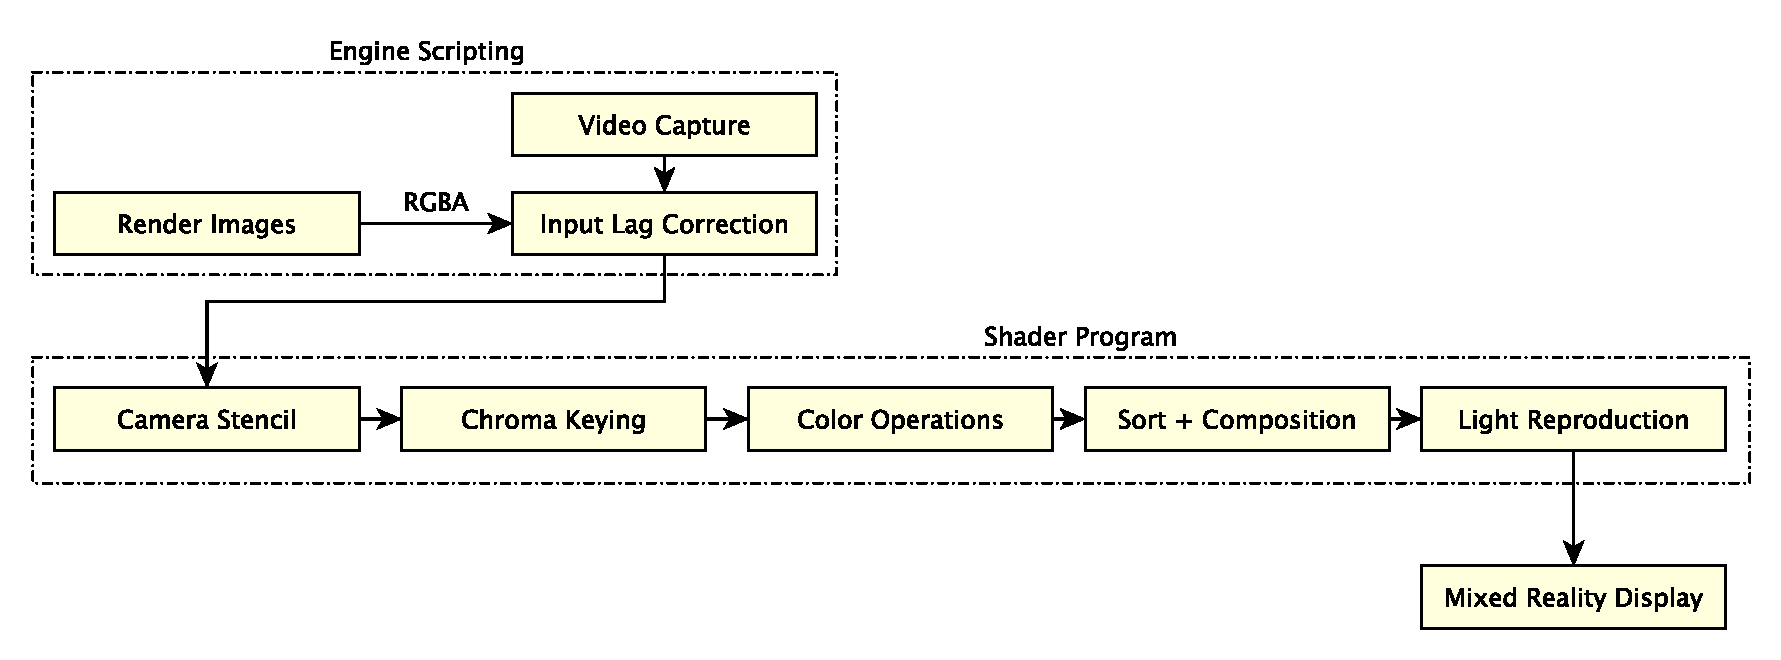
\includegraphics[width=\textwidth]{_raw_resources/pipeline_steps/4_9_order_alt.pdf}
	\caption{Actual order of computation}
	\label{fig:steps:order:alt}
\end{figure}

\todo[inline]{This might be appendix-worthy - then move a note to the chapters' 
beginning.}